\chapter{Urban Source Identification Results and Discussion}

% Compare how well we identify shielded/unshielded isotopes when training set has shielding, doesn't have shielding. 

% Compare how well we identify isotopes over different distances if training set has one vs many distances

% Compare how well we identify isotopes with different calibration sampling granularity 


\section{Problem Description and Training Dataset Overview}

This chapter applies machine learning algorithms to solve the problem of a identifying a radioactive source in an urban environment where a source may be present. This scenario is applicable when performing source interdiction searching cargo containers, vehicles at boarder crossings, or security at high profile events. Urban environments present unique challenges to gamma-ray spectroscopy. Background radiation can change over city blocks due to different concentrations of uranium and thorium in building materials. Sources may be purposely shielded by unknown amounts of material to obscure their gamma-ray signal.


\subsection{Training Dataset Overview}

The datasets used to train the models are composed of noiseless simulated gamma-ray templates. A one-dimension particle transport code developed at Sandia National Laboratory, GADRAS-DRF, was used to generate these templates. This simulation code can be used to model the conditions that effect spectra. The parameters used in this study are different detector materials, detector size, environmental scattering factors, shielding, and background as a function of location. GADRAS-DRF includes an option to create spectra without the Poisson noise expected for a spectrum. Using this, noiseless templates were generated.


Table 



Spectra change due to changes in measurement geometry. These changes include source-to-detector distance and the distance of both the detector and source from objects in an environment. To demonstrate this effect, $^{60}$Co spectra were simulated, Figure \ref{fig:sim_spectra_distance_comparison}, with different source-to-detector distances.

$^{60}$Co spectra were also simulated at different distances from the ground, shown in Figure \ref{fig:sim_spectra_height_comparison}.



\begin{figure}[H]
\centering
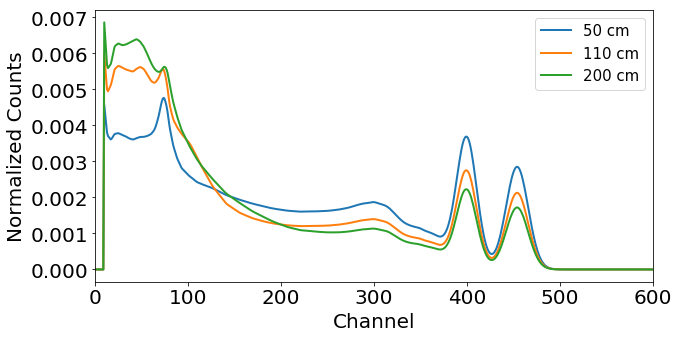
\includegraphics[width=0.95\linewidth]{images/sim_spectra_distance_comparison}
\caption{Comparison of a $^{60}$Co spectrum simulated at various source-detector distances.}
\label{fig:sim_spectra_distance_comparison}
\end{figure}

\begin{figure}[H]
\centering
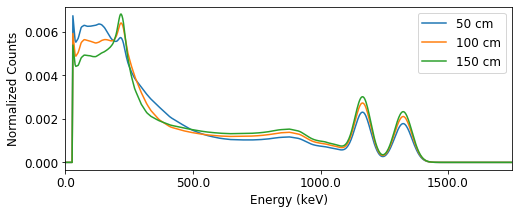
\includegraphics[width=0.95\linewidth]{images/sim_spectra_height_comparison}
\caption{Comparison of a $^{60}$Co spectrum simulated at various source-detector heights off the ground.}
\label{fig:sim_spectra_height_comparison}
\end{figure}



To incorporate these changes, templates simulated at different distances are included in the dataset. These distances start at 30cm, which is the distance at which a 1 uCi source will have an activity of about 400 cps on a 2 inch diameter detector. This is about twice the expected activity of background. 

Changes in calibration due to temperature shifts are also considered. Due to the relatively large magnitude in calibration shifts due to temperature shifts from -5 C to 40 C, it is expected incorporating these additions will also make the algorithm robust against calibration. If a As seen in \ref{fig:CASANOVAS2012588}, 


Spectra are also simulated with different FWHM parameters.


\begin{figure}[H]
\centering
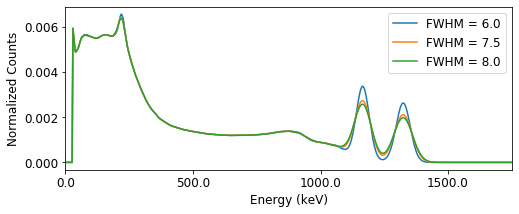
\includegraphics[width=0.95\linewidth]{images/sim_spectra_FWHM_comparison}
\caption{Comparison of a $^{60}$Co spectrum simulated with various FWHM parameters.}
\label{fig:sim_spectra_FWHM_comparison}
\end{figure}


\section{Data Augmentation Used}

Several data augmentation techniques are employed when training the 



\section{Training the Dense and Convolution Autoencoder}

The DAE and CAE are trained to act as feature extractors. There are a number of ways to construct the input and output for a spectral autoencoder. 





\section{Model Evaluation}

\subsection{Model performance on the easy dataset}


\begin{figure}[H]
	\centering
	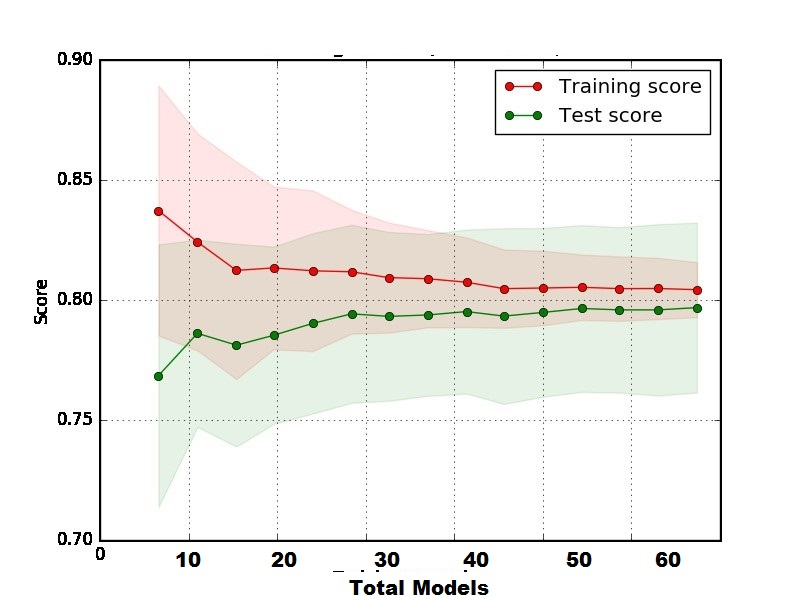
\includegraphics[width=0.9\linewidth]{model_choice_hyperparameter_search_images/asymptotic_performance_dummy}
	\caption{Model performance on the easy dataset. }
	\label{fig:asymptotic_performance}
\end{figure}

















% \section{Results from training all models}

% When training final models, two main questions need to be addressed: how good is a given architecture at solving a problem on its training dataset and how good is a given dataset at generalizing to outside examples.

% To determine how good a given architecture solves a problem, asymptotic convergence of the models performance needs to be measured. Because of the inherent stochastic nature of training machine learning algorithms (different random weight initialization, different mini-batches chosen during training, different data augmentation manifestations), each time a new network is trained the networks parameters and results will differ. This means a single trained instance of some model A may outperform a single trained instance of model B by chance, despite model B being an overall superior architecture. To more realistically compare how models perform on some dataset, a number of networks can be trained and their average performance compared. This is a method called bagging.

% \subsection{Asymptotic Model Performance on Training Dataset}

% For the best DNN and CNN architectures found in the hyperparameter search, using 'enough' data data samples as found in the hyperparameter search, 30 networks are trained. Their performance is observed in Figure \ref{fig:asymptotic_performance}.


%% Can also include performance using templates with extreme augmentation
% \begin{figure}[H]
% 	\centering
% 	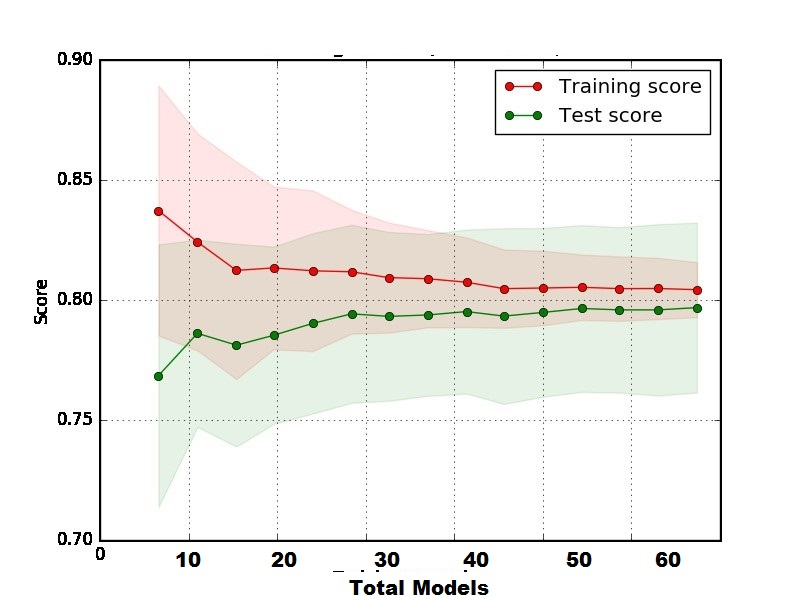
\includegraphics[width=0.8\linewidth]{model_choice_hyperparameter_search_images/asymptotic_performance_dummy}
% 	\caption{Asymptotic model performance for both the CNN and DNN on the training sets.}
% 	\label{fig:asymptotic_performance}
% \end{figure}

% Using N models as representative of asymptotic performance, justified in Figure \ref{fig:asymptotic_performance}, we can check out the confusion matrix associated with the test dataset to gain insight into how the algorithm is performing poorly and predict future shortcomings.


%% Can also include performance using templates with extreme augmentation
% \begin{figure}[H]
% 	\centering
% 	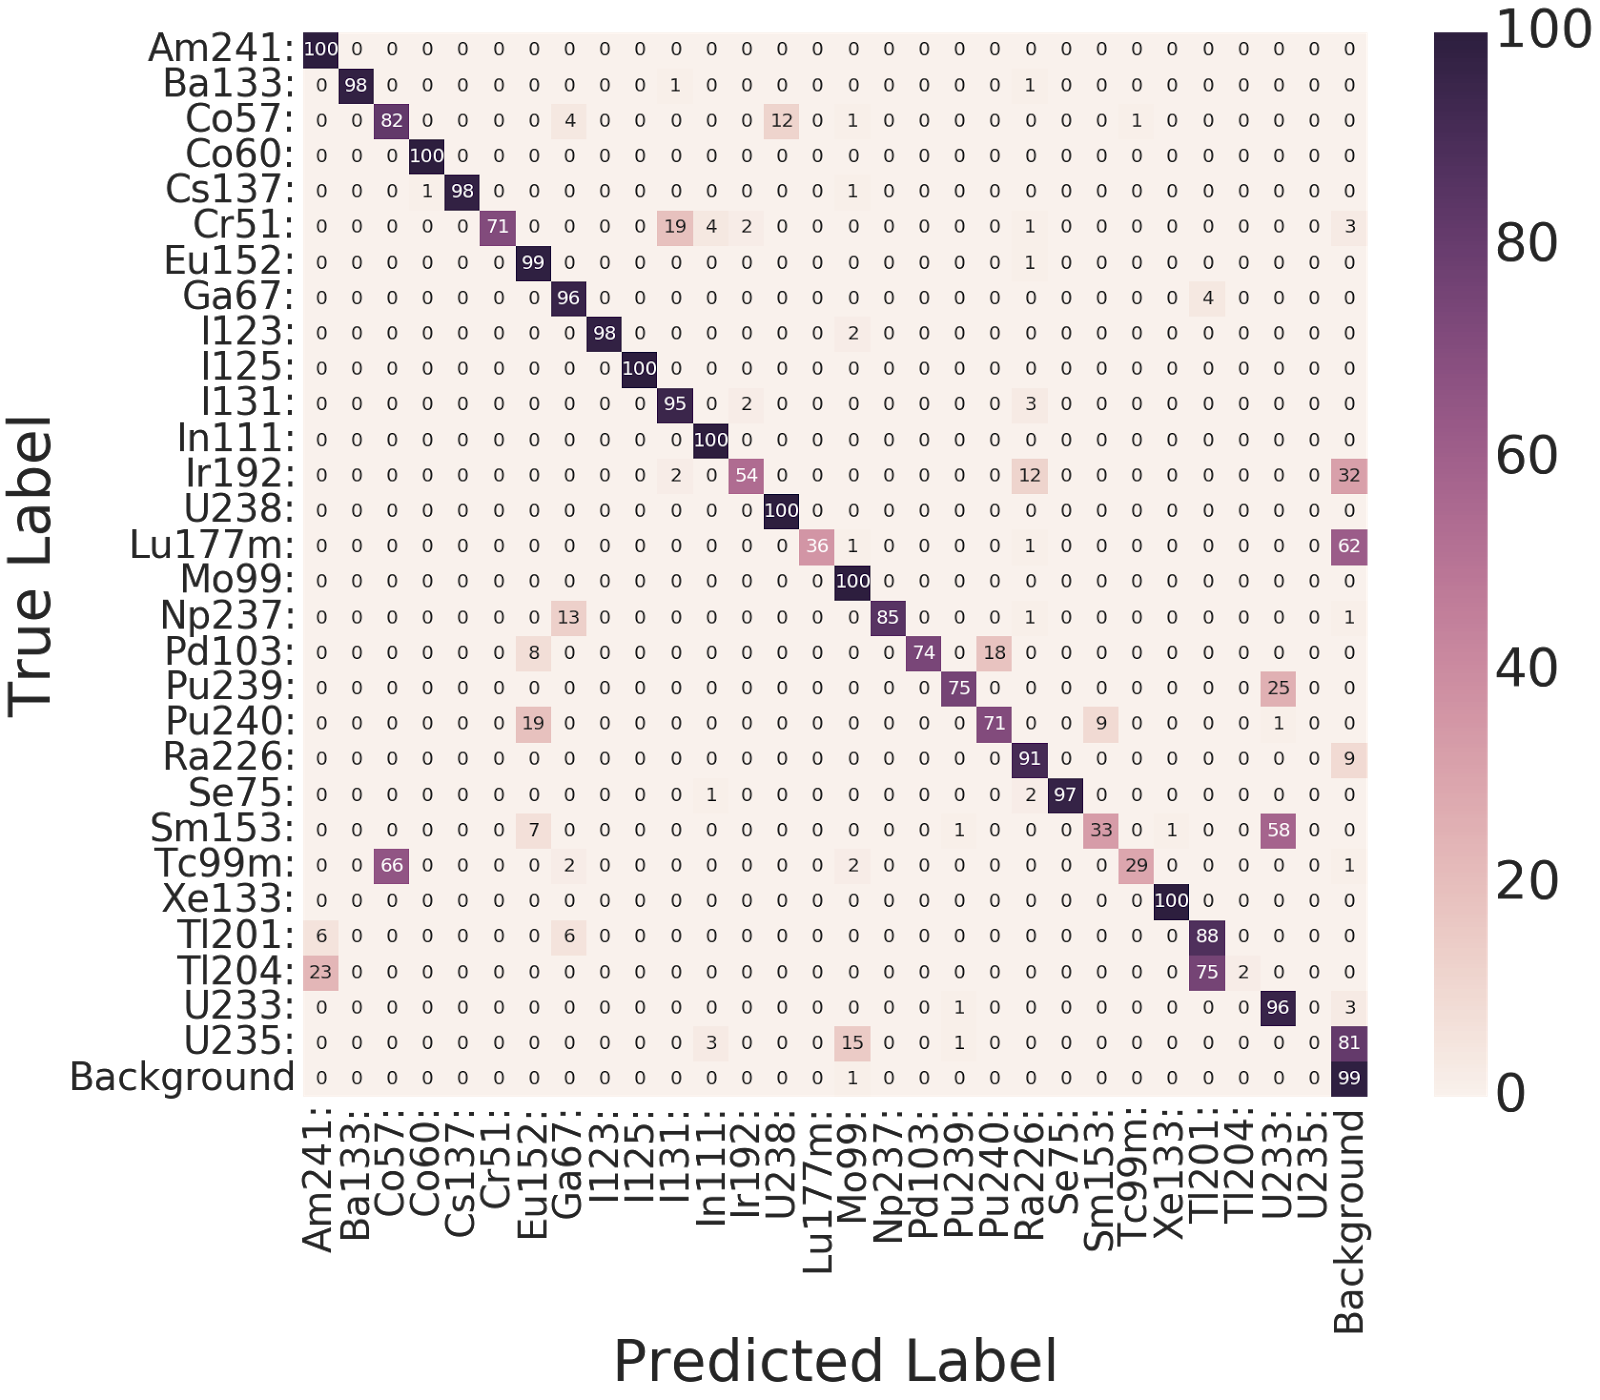
\includegraphics[width=0.8\linewidth]{model_choice_hyperparameter_search_images/conf_matrix_example}
% 	\caption{Asymptotic model performance for both the CNN and DNN on the training sets.}
% 	\label{fig:asymptotic_performance}
% \end{figure}

% Can also analyze how changing a threshold would affect precision/recall!

% \subsection{Results from training models using extreme data augmentation vs Data Augmentation grid sampling}

% Show learning curve between models 
% Instead of training examples on x-axis, plot against "number of divisions" (which also has a number of training examples included...)
% Note! You can start holding parameters constant to see what parameter the model is having difficulty explaining
% \begin{figure}[H]
%	\centering
%	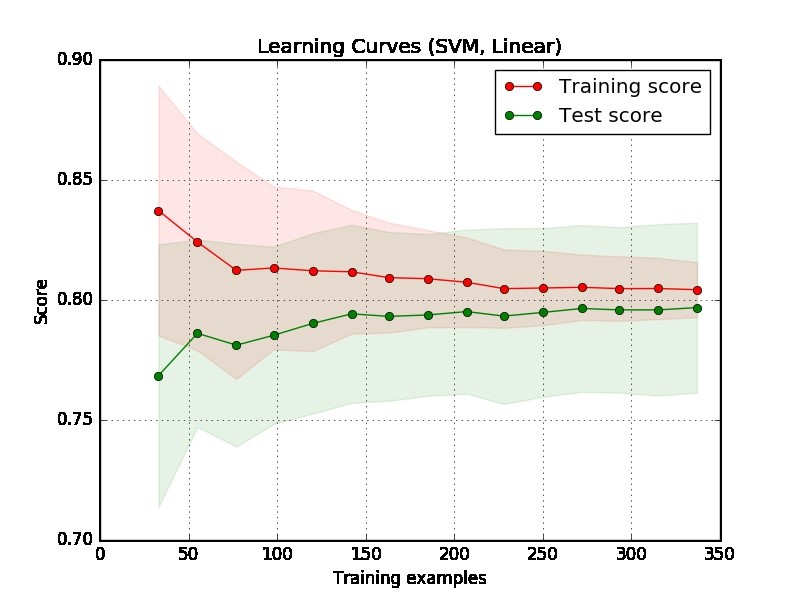
\includegraphics[width=0.8\linewidth]{model_choice_hyperparameter_search_images/learning_curve_dummy}
%	\caption{Learning curve example.}
%	\label{fig:Node}
%\end{figure}

%% Plot of average F1-score vs epochs for all models. Datasets include different detector model (use this as validation set) and same detector model with certain augmentation parameters frozen (or just the training set).


%% Plot of average F1-score vs epochs for all models. Datasets include different detector model (us this as validation set) and same detector model with certain augmentation parameters frozen (or just the training set).

\subsection{Results on Spectra for ANSI compliance}

This section shows model asymptotic performance vs integration time for ANSI compliance. Using N models (justified previously as asymptotic). 


% List Represents table of 
\begin{itemize}
  \item $^{137}$Cs + depleted uranium (DU)
  \item $^{99m}$Tc + HEU
  \item $^{201}$Tl + HEU
  \item $^{67}$Ga + HEU
  \item $^{131}$I + WGPu
  \item Naturally occurring radioactive material (NORM) + HEU
  \item NORM + WGPu
\end{itemize}


\subsection{Results on Measured Spectra}

This section shows model asymptotic performance vs integration time for a few different settings (different voltages, shielding)

To investigate how each model identified real spectra behind shielding and spectra with different calibrations, real spectra were measured. Sources include $^{137}$Cs, $^{60}$Co, $^{133}$Ba, and $^{152}$Eu. 


\subsubsection{Asymptotic Model Performance on Changing Voltage}

To see the generalization performance of the model to changing calibration, spectra with different voltages are recorded and their asymptotic performance compared.

Spectra were measured with different detector calibrations. A 2x2 Ortec NaI detector was set to 770 V, setting it's 1024th channel to 3 MeV. To capture a large range of calibrations, voltages varied from 720 V to 820 V in steps of 15 V. The $^{137}$Cs, $^{60}$Co, and $^{133}$Ba source had an activity of 1$\mu$C. For these sources, a source-to-detector distance of 14.25 mm was used to keep the cps on the detector from the source equal to the cps on the detector from background.

Figures \ref{fig:model_asymptotic_performance_co60} and \ref{fig:model_asymptotic_performance_cs137} show performance for isotopes with comparatively simple spectra.

\begin{figure}[H]
	\centering
	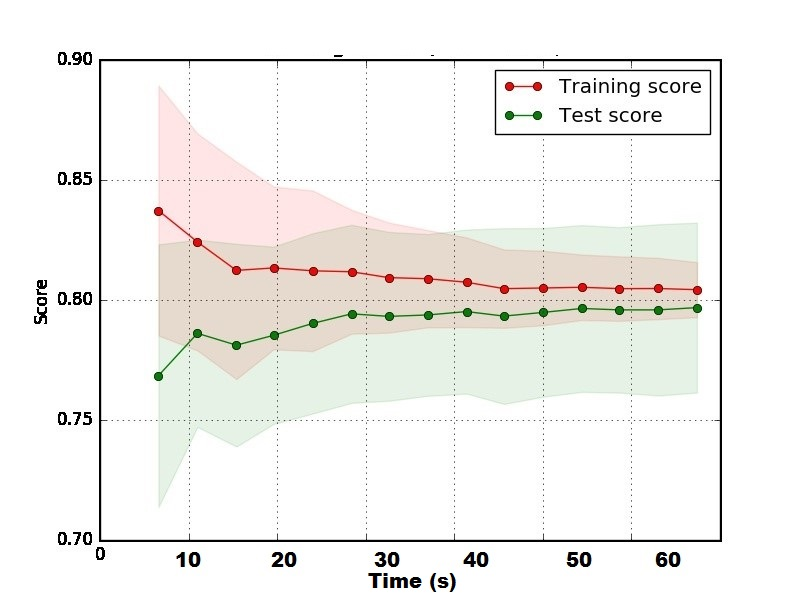
\includegraphics[width=0.75\linewidth]{model_choice_hyperparameter_search_images/asymptotic_performance_time}
	\caption{Asymptotic model performance for both the CNN and DNN on voltage vs integration time for $^{60}$Co.}
	\label{fig:model_asymptotic_performance_co60}
\end{figure}

\begin{figure}[H]
	\centering
	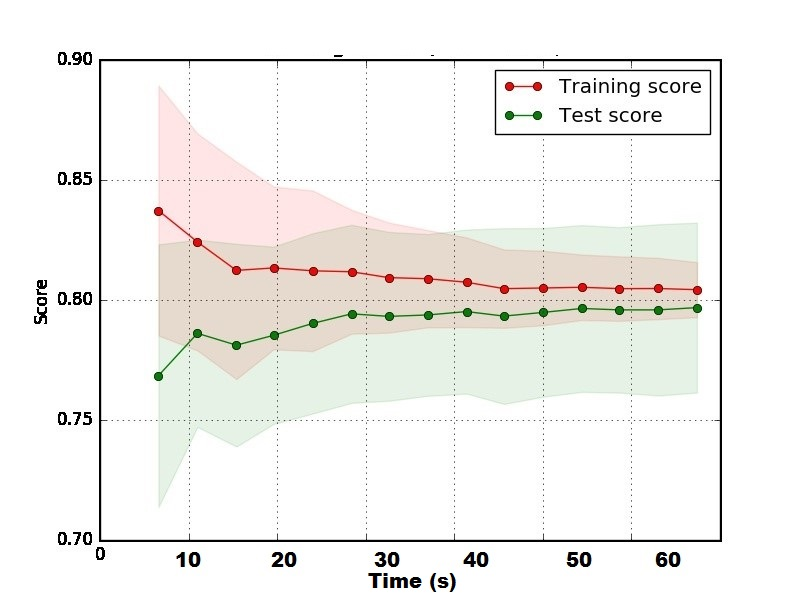
\includegraphics[width=0.75\linewidth]{model_choice_hyperparameter_search_images/asymptotic_performance_time}
	\caption{Asymptotic model performance for both the CNN and DNN on voltage vs integration time for $^{137}$Cs.}
	\label{fig:model_asymptotic_performance_cs137}
\end{figure}

Figures \ref{fig:model_asymptotic_performance_eu152} and \ref{fig:model_asymptotic_performance_ba133} show performance for isotopes with comparatively complicated spectra.

\begin{figure}[H]
	\centering
	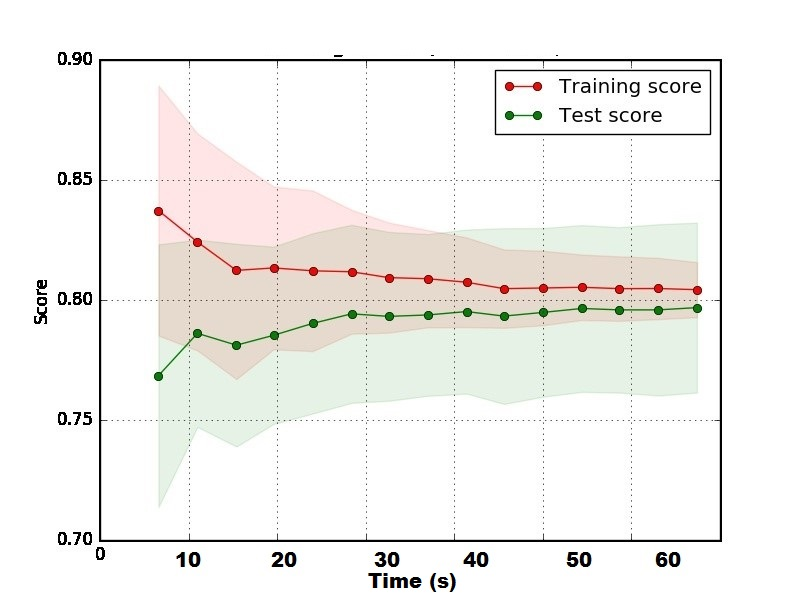
\includegraphics[width=0.75\linewidth]{model_choice_hyperparameter_search_images/asymptotic_performance_time}
	\caption{Asymptotic model performance for both the CNN and DNN on voltage vs integration time for $^{152}$Eu.}
	\label{fig:model_asymptotic_performance_eu152}
\end{figure}

\begin{figure}[H]
	\centering
	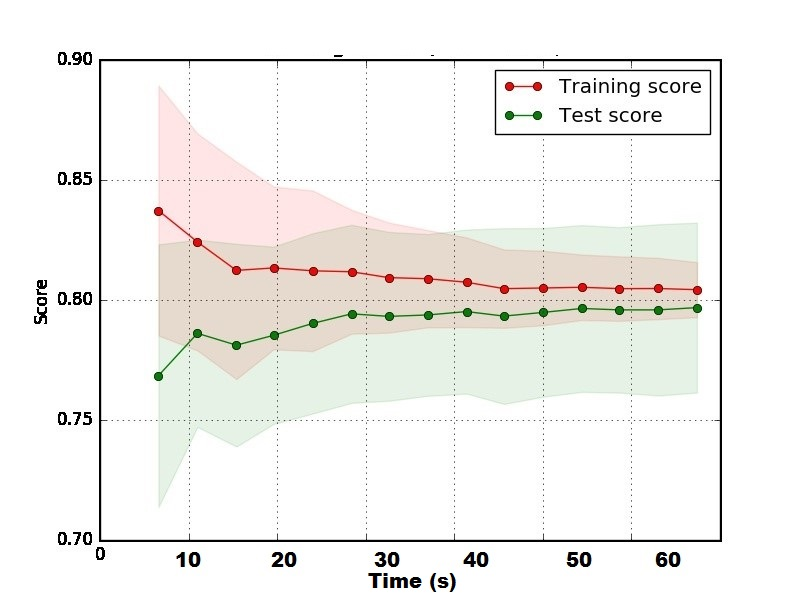
\includegraphics[width=0.75\linewidth]{model_choice_hyperparameter_search_images/asymptotic_performance_time}
	\caption{Asymptotic model performance for both the CNN and DNN on voltage vs integration time for $^{133}$Ba.}
	\label{fig:model_asymptotic_performance_ba133}
\end{figure}

\subsubsection{Asymptotic Model Performance on Changing Shielding}

\begin{figure}[H]
	\centering
	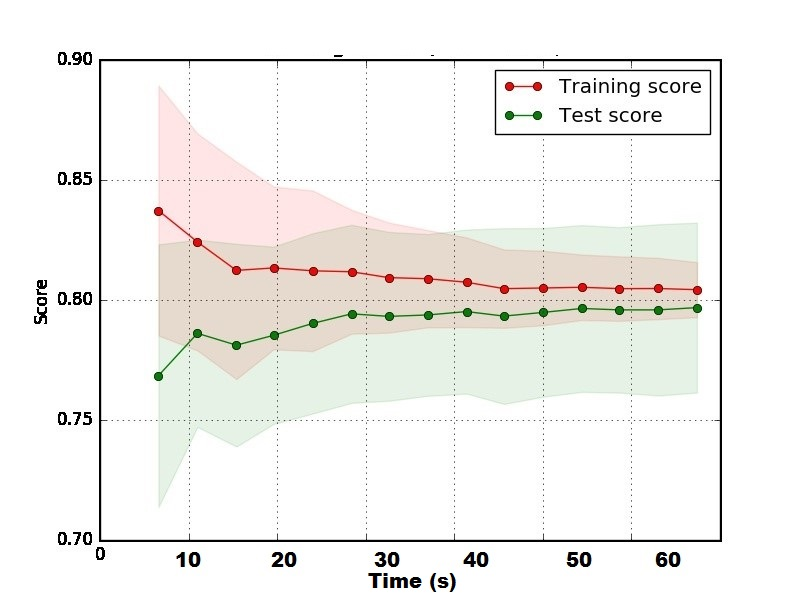
\includegraphics[width=0.75\linewidth]{model_choice_hyperparameter_search_images/asymptotic_performance_time}
	\caption{Asymptotic model performance for both the CNN and DNN on shielding vs integration time.}
	\label{fig:asymptotic_performance}
\end{figure}



\subsubsection{Spectra with a Single Isotope}




\subsubsection{Spectra with a Isotope Mixtures}

% Super crazy, check out effect of changing ID threshold on F1 score for these data. Or, using optimum threshold found before, check out 

The ANNs ability to identify mixtures of less than three isotopes will be addressed. Mixtures of $^{60}$Co, $^{137}$Cs, $^{152}$Eu, and $^{133}$Ba will be recorded. The mean ANN outputs and their variances will be reported.
